\documentclass[13pt, usenames,dvipsnames]{beamer} % \usepackage[defaultmono]{droidmono}
% \renewcommand*\familydefault{\ttdefault} %% Only if the base font of the document is to be typewriter style
% \usepackage[T1]{fontenc}
% \makeatletter
% \input droid/t1fdm.fd
% \makeatother

\usepackage[T1]{fontenc}
\usepackage{lmodern}
\usepackage{minted}
\usepackage{xcolor}
\usepackage{etoolbox}
\usepackage{tikz}
\usetikzlibrary{fit}
\usepackage{color, colortbl}
\usepackage{soul}
\usepackage{fontspec}
\usepackage{fontawesome}
\usepackage{array}
\usepackage{hyperref}
\usepackage{transparent}

% \usepackage[export]{adjustbox}

\usetikzlibrary{mindmap,trees,shadows,shapes,positioning,arrows,calc,matrix}
\tikzset{
  invisible/.style={opacity=0},
  visible on/.style={alt={#1{}{invisible}}},
  alt/.code args={<#1>#2#3}{%
    \alt<#1>{\pgfkeysalso{#2}}{\pgfkeysalso{#3}} % \pgfkeysalso doesn't change the path
  },
}
\setmonofont[
  Contextuals={Alternate}
  ]{FiraCode-Regular}




\definecolor{aliceblue}{rgb}{0.94, 0.97, 1.0}
\definecolor{beige}{rgb}{0.96, 0.96, 0.86}
\definecolor{chartreuse}{rgb}{0.87, 1.0, 0.0}


\sethlcolor{yellow}

\usemintedstyle{manni}
\setminted{fontsize=\footnotesize, baselinestretch=1}

\setbeamertemplate{footline}[frame number]
\setbeamercolor{normal text}{fg=black!80,bg=white}

%gets rid of bottom navigation bars
\setbeamertemplate{footline}[frame number]{}

%gets rid of navigation symbols
\setbeamertemplate{navigation symbols}{}

\newcommand{\mycode}[2][\tiny] {\mintinline[bgcolor=gray!10, fontsize=#1]{python}{#2}}

\title{Parallel Computing in Python}
\subtitle{Current State and Recent Advances}
\author{\href{http://kbroman.org}{Pierre Glaser, INRIA}
\href{https://github.com/pierreglaser}{\faGithub}
\href{https://twitter.com/pierreglaser}{\faTwitter}}
\titlegraphic{
    \begin{columns}
        \begin{column}{0.7\textwidth}
    \includegraphics[width=3cm]{media/inria-logo.png}
        \end{column}
        \begin{column}{0.3\textwidth}
       \includegraphics[width=3cm]{media/logo_parietal.png}
        \end{column}
    \end{columns}
   }


\begin{document}
\begin{frame}[fragile]{}
    \titlepage
\end{frame}

\vspace{3em}

\begin{frame}[t]{}
    \center
    \vspace{7em}
    \begin{itemize}
        \setlength\itemsep{1em}
        \item[]\textbf{Parallel computing in machine learning - an overview }
        \item[]\textbf{Built-in and Third Party multiprocessing ressources}
        \item[]\textbf{Optimizing data communication}
    \end{itemize}
\end{frame}


\section{Parallel computing in machine learning - an overview}
    \begin{frame}[t]{}
        \vspace{10em}
        \centering{\large \textbf{Parallel computing in machine learning - an overview}}
    \end{frame}
    \subsection{Python? }

    \begin{frame}[t]{Python? What for?}
        \setbeamercolor{block body}{bg=gray!80}
        \setbeamercolor{frametitle}{bg=gray!80}
        \setbeamercolor{block title}{bg=gray!80}
        \begin{figure}[htpb]
            \vspace*{-0.5cm}
            \hspace*{-1.0cm}
            \alt<2>{\includegraphics[width=1\linewidth]{media/psf_usage_survey_highlighted.png}}{\includegraphics[width=1\linewidth]{media/psf_usage_survey.png}}
            \vspace*{-0.5cm}
            \label{fig:media/better_screenshot_python_development_results}
        \end{figure}
        \centering{Python usage among developers
    \footnote{\tiny source: https://www.jetbrains.com/research/python-developers-survey-2018/}
        }
    \end{frame}

    \begin{frame}{A growing data science ecosystem}
        \uncover<1->{
        \begin{tabular}{m{1cm} m{5cm} m{3cm}}
            & \\
            \includegraphics[width=\linewidth]{media/numpy-logo.png} & numpy
            for n-dimensional arrays &
            \includegraphics[scale=0.4]{media/used_by_numpy.png} \\
        \end{tabular}
        }
        \uncover<2->{
        \begin{tabular}{m{1cm} m{5cm} m{3cm}}
            \includegraphics[width=\linewidth]{media/pandas.png} & pandas for
            data analytics &
            \includegraphics[scale=0.4]{media/used_by_pandas.png} \\

        \end{tabular}
        }
        \uncover<3->{
        \begin{tabular}{m{1cm} m{5cm} m{3cm}}
            \includegraphics[width=\linewidth]{media/scikit-learn-logo.png} &
            scikit-learn for machine learning &
            \includegraphics[scale=0.4]{media/used_by_scikit-learn.png} \\
            \\
        \end{tabular}
        }
        % \begin{tikzpicture}
        % \node[align=left] (inst) at (1, 0) {%
        % \node[align=left] (inst) at (1, -1) {%
        % \includegraphics[scale=0.4]{media/used_by_scikit-learn.png}};
        % \node[align=left] (inst) at (8.5, 0) {%
        % \includegraphics[scale=0.30]{media/numpy-logo.png}};
        % \node[align=left] (inst) at (8.5, -1.5) {%
        % \includegraphics[scale=0.4]{media/used_by_numpy.png}};
        % \node[align=left] (inst) at (4.5, -3) {%
        % \includegraphics[scale=0.40]{media/pandas.png}};
        % \node[align=left] (inst) at (4.5, -4.3) {%
        % \includegraphics[scale=0.4]{media/used_by_pandas.png}};
        % \end{tikzpicture}
    \end{frame}

    \begin{frame}[t]{Parallel computing? Why?}
        \vspace{1cm}
        \textbf{Independent, similar computation} happens a lot in machine learning. We
        call it embarassingly parallel tasks. Famous examples:
        \vspace{1cm}
        \begin{itemize}
            \item<2-> cross validation
            \item<2-> random forests
            \item<2-> hyperparameter selection using grid search
        \end{itemize}
        \vspace{1cm}
        \uncover<2>{
        \begin{flushright}
            \small
        Happens for many scikit-learn estimators, but not all.
        \end{flushright}
    }
    \end{frame}

    \begin{frame}[fragile]{Parallel computing in scikit-learn made easy}
        % \small
        Parallelization in \mycode[\small]{scikit-learn}:
        \vspace{1em}
        \begin{itemize}
            \setlength\itemsep{1em}
            \item<1-> ubiquituous
            \item<1-> painlessly toggled using estimators's \mycode[\small]{n_jobs} option:
        \end{itemize}
        \uncover<2->{
        \inputminted[fontsize=\scriptsize,bgcolor=beige]{python}{scripts/logistic_regression.py}
        }
    \end{frame}

    \begin{frame}[fragile]{Multithreading or multiprocessing?}
        Parallelism usually exist under two different forms:
        \vspace{1em}
        \uncover<2>{
        \begin{itemize}
            \setlength\itemsep{1em}
            \item executing  multiple processes (python programs) in parallel
            \item executing multiple threads of a same process in parallel
        \end{itemize}
        }
    \end{frame}

    \begin{frame}[t]{Fitting a random forest}
        \footnotesize
        \begin{flushright}
        I want to fit many small decision trees independently, on the same data.
        \end{flushright}
        \vspace{1cm}
        \begin{columns}
            \begin{column}{0.5\textwidth}
                \only<2-5>{%
                    \small \textbf{thread-based parallelism:} \\
                \footnotesize
                \vspace{0.5cm}
                +: threads share memory
                \begin{itemize}
                    \item no data copies
                    \item no data transfer
                \end{itemize}
                \vspace{0.2cm}
                -: By default, Python forces threads to run sequentially\\
                The GIL can be released when calling native code
                (\mycode{numpy}, \mycode{scipy}...)
                }
                \only<6->{%
                \scriptsize
                    \small \textbf{process-based parallelism:} \\
                    \footnotesize
                \vspace{0.5cm}
                +: processes are assured to run in parallel
                \vspace{0.2cm} \\
                -: need to pass and copy data around
                \begin{itemize}
                    \item larger memory footprint
                    \item data transfer overhead
                \end{itemize}
                }
                \vspace{2.3cm}
            \end{column}
            \begin{column}{0.6\textwidth}
                \begin{tikzpicture}[scale=0.55]
                    \tikzset{rounded corners=1}
                \node[align=left, visible on=<2->] (main-thread) at (5, 5.7) {%
                        \only<2-5>{\mycode{main thread}}
                        \only<6->{\mycode{main process}}};
                \node[align=left, visible on=<2>] (all) at (5, 4) {%
                    \resizebox{0.13\textwidth}{!}{%
                    \begin{tabular}{c c}
                        a & b \\
                        \hline
                        \hline
                        1 & 2 \\
                        3 & 4 \\
                        5 & 6 \\
                        7 & 8 \\
                \end{tabular}}};
                \node[align=left, visible on=<3>] (all) at (5, 4) {%
                    \resizebox{0.13\textwidth}{!}{%
                    \begin{tabular}{c c}
                        a & b \\
                        \hline
                        \hline
                        % \rowcolor{beige}
                        1 & 2 \\
                        3 & 4 \\
                        % \rowcolor{beige}
                        5 & 6 \\
                        % \rowcolor{beige}
                        7 & 8 \\
                \end{tabular}}};
                \node[align=left, visible on=<4>] (all) at (5, 4) {%
                    \resizebox{0.13\textwidth}{!}{%
                    \begin{tabular}{c c}
                        a & b \\
                        \hline
                        \hline
                        1 & 2 \\
                        % \rowcolor{aliceblue}
                        3 & 4 \\
                        % \rowcolor{aliceblue}
                        5 & 6 \\
                        % \rowcolor{aliceblue}
                        7 & 8 \\
                \end{tabular}}};
                \node[align=left, visible on=<5>] (all) at (5, 4) {%
                    \resizebox{0.13\textwidth}{!}{%
                    \begin{tabular}{c c}
                        a & b \\
                        \hline
                        \hline
                        % \rowcolor{chartreuse}
                        1 & 2 \\
                        % \rowcolor{chartreuse}
                        3 & 4 \\
                        % \rowcolor{chartreuse}
                        5 & 6 \\
                        7 & 8 \\
                \end{tabular}}};
                \node[align=left, visible on=<6->] (all) at (5, 4) {%
                    \resizebox{0.13\textwidth}{!}{%
                    \begin{tabular}{c c}
                        a & b \\
                        \hline
                        \hline
                        1 & 2 \\
                        3 & 4 \\
                        5 & 6 \\
                        7 & 8 \\
                \end{tabular}}};
                \node[align=left, visible on=<7->] (cv1) at (1.5, 0) {%
                    \uncover<-7>{
                    \resizebox{0.13\textwidth}{!}{%
                        \begin{tabular}{c c}
                            a & b \\
                            \hline
                            \hline
                            % \rowcolor{beige}
                            1 & 2 \\
                            3 & 4 \\
                            % \rowcolor{beige}
                            5 & 6 \\
                            % \rowcolor{beige}
                            7 & 8 \\
                    \end{tabular}}}};
                \node[align=left, visible on = <7->] (cv2) at (5, 0) {%
                    \uncover<-7>{
                    \resizebox{0.13\textwidth}{!}{%
                    \begin{tabular}{c c}
                        a & b \\
                        \hline
                        \hline
                        % \rowcolor{aliceblue}
                        1 & 2 \\
                        3 & 4 \\
                        % \rowcolor{aliceblue}
                        5 & 6 \\
                        % \rowcolor{aliceblue}
                        7 & 8 \\
                \end{tabular}}}};
                \node[align=left, visible on=<7->] (cv3) at (8.5, 0) {%
                    \uncover<-7>{
                    \resizebox{0.13\textwidth}{!}{%
                        \begin{tabular}{c c}
                            a & b \\
                            \hline
                            \hline
                            % \rowcolor{chartreuse}
                            1 & 2 \\
                            % \rowcolor{chartreuse}
                            % \rowcolor{chartreuse}
                            3 & 4 \\
                            5 & 6 \\
                            7 & 8 \\
                \end{tabular}}}};
                \node[align=left, visible on = <2->] (worker3) at (8.5, 1.6){%
                % \only<-4>{\mycode{Thread-3}}};
                \temporal<6-7>{\mycode{Thread-3}}{\mycode{Process-3}}{\mycode{Process-3}}};

                \node[align=left, visible on = <2-8>] (worker2) at (5, 1.6){%
                % \only<-4>{\mycode{Thread-2}}};
                \temporal<6-7>{\mycode{Thread-2}}{\mycode{Process-2}}{\mycode{Process-2}}};

                \node[visible on = <2->] (worker1) at (1.5, 1.6){%
                % \only<-4>{\mycode{Thread-1   }}};
                    % \only<-4>{\mycode{Thread-1   }}
                    % \only<-4>{\mycode{Thread-1   }}
                \temporal<6-7>{\mycode{Thread-1}}{\mycode{Process-1}}{\mycode{Process-1}}};
                % {\draw[->, visible on=<5->] (all.south)--(cv1.north east);}
                % {\draw[->, visible on=<6->] (all.south)--(cv2.north);}
                % {\draw[->, visible on=<7->] (all.south)--(cv3.north west);}
                {\draw[->, visible on=<3>] (worker1.east)--(all.south);}
                {\draw[->, visible on=<4>] (worker2.north)--(all.south);}
                {\draw[->, visible on=<5>] (worker3.west)--(all.south);}
                % {\draw[->, visible on=<3->] (all.south)--(cv2.north);}
                % {\draw[->, visible on=<4->] (all.south)--(cv3.north west);}
                \node[visible on =<2-5>, draw,inner sep=5mm,fit=(all) (worker2) (worker3) (worker1)] {};
                \node[visible on =<6->, draw,inner sep=0.5mm,fit=(main-thread) (all) (all) (all)] {};
                \node[visible on =<7->, draw,inner sep=0.5mm,fit=(worker1) (cv1) (cv1) (cv1)] {};
                \node[visible on =<7->, draw,inner sep=0.5mm,fit=(worker2) (cv2) (cv2) (cv2)] {};
                \node[visible on =<7->, draw,inner sep=0.5mm,fit=(worker3) (cv3) (cv3) (cv3)] {};


                \node[align=center, dotted, draw, rectangle,
                above right =0.7cm and -1cm of cv3, visible on =<8->] (memmaparray) {%
                    \tiny memmaped data \\
                    \resizebox{0.13\textwidth}{!}{%
                    \begin{tabular}{c c}
                        a & b \\
                        \hline
                        \hline
                        1 & 2 \\
                        3 & 4 \\
                        5 & 6 \\
                        7 & 8 \\
                    \end{tabular}}};
                % \node[align=center, above=0.1cm of memmaparray]
                % (legendmemap) {\tiny memmaped\\ \tiny data};
                % \draw node[rectangle,  draw=gray, font=\tiny] (main){memmaped};
                \path[->, visible on = <8>] (main-thread.north) edge[bend left]
                (memmaparray.north);

                \node[visible on = <6->, align=left] (legend) at (4, -3){};
                \node[visible on= <6->, draw,inner sep=1mm,fit=(legend) (legend) (legend) (legend)] {};
                \node[visible on = <6->, align=left] (title) at (7, -3){\tiny : single python interpreter};

                \end{tikzpicture}
            \end{column}
        \end{columns}
    \end{frame}

    \begin{frame}[t]{In practice}
        \vspace*{-1.3cm}
        \begin{figure}[htpb]
            \centering
            \only<1>{\includegraphics[width=\linewidth]{media/plots/benchmark_plots/seq_vs_parallel_bounds_only.png}}%
            \only<2>{\includegraphics[width=\linewidth]{media/plots/benchmark_plots/seq_vs_parallel_bounds_and_scatter.png}}%
            \only<3>{\includegraphics[width=\linewidth]{media/plots/benchmark_plots/seq_vs_parallel_bounds_and_scatter_and_patches.png}}
            \caption{Model fitting time - parallel vs. sequential}
            \label{seq_vs_parallel_bounds_only}
        \end{figure}
    \end{frame}

    % \begin{frame}[fragile]{takeway - processes vs. threads}
    %     \begin{tabular}{m{0.5cm} m{10cm}}
    %         \includegraphics[width=\linewidth] {media/lock-emoji.png} &
    %         \textit{thread-based parallelism} is useful only if the compute-heavy part
    %         of your program releases \mycode{Python}'s GIL. This is not
    %         something parallel computing libraries have a say on. \\
    %     \end{tabular}
    %     \vspace{1em}

    %     \uncover<2->{
    %     \begin{tabular}{m{0.5cm} m{10cm}}
    %         \includegraphics[width=\linewidth] {media/unlocked-lock-emoji.png} &
    %         \textit{process-based parallesim} guarantees parallel execution of
    %         \mycode{Python} code, but this comes at the cost of \textcolor{red}{transfering
    %         data} to the newly-created processes
    %     \end{tabular}
    %     }
    % \end{frame}


\section{Built-in and Third Party multiprocessing ressources}
    \begin{frame}[t]{}
        \vspace{10em}
        \centering{\large \textbf{Built-in and Third Party multiprocessing
        ressources}}
    \end{frame}



    \subsection{In the Standard Library}

    \begin{frame}[fragile]{\mycode[\small]{multiprocessing}}
        provides all necessary constructs for creating and handling proccesses
        in \mintinline[bgcolor=gray!10]{python}{Python} programs
        \vspace{1em}
        \begin{columns}
            \begin{column}{0.5\textwidth}
                \begin{itemize}
                    \visible<2->{\item creation}
                    \visible<3->{\item communication}
                    \visible<4->{\item \hl{synchronization}}
                \end{itemize}
                \vspace{2cm}
            \end{column}
            \begin{column}{0.5\textwidth}
                \begin{tikzpicture}
                    \tikzset{rounded corners=1}
                \draw (0, 0) node[rectangle, visible on=<2->, draw=gray, font=\tiny] (main){main process};
                \draw (0, -4) node[rectangle, visible on=<4->, draw=gray, font=\tiny,alt=<4>{fill=yellow}{fill=gray!10} ]
                    (lock){\mintinline[fontsize=\tiny]{python}{mp.Lock}};
                \draw (1.5, -3) node[rectangle, visible on = <2->, draw=gray, font=\tiny,alt=<2>{fill=yellow}{fill=gray!10} ]
                    (child2){\mintinline[fontsize=\tiny]{python}{mp.Process}};
                \draw (-1.5, -3) node[rectangle, draw=gray,visible on = <2->, font=\tiny,alt=<2>{fill=yellow}{fill=gray!10} ]
                    (child1){\mintinline[fontsize=\tiny]{python}{mp.Process}};
                % \draw (0, -2) node[rectangle, inner sep=1pt, draw=gray, font=\tiny] (queue){child process};
                \draw (0, -1.5) node[rectangle split, visible on=<3->, rectangle split parts=3,
                       draw, minimum width=1cm,font=\small,
                      rectangle split part align={center}, inner sep=1pt,
                      alt=<3>{fill=yellow}{}]
                      (queue) {};
                  \draw (2, -1.5) node[visible on=<3->, alt=<3>{fill=yellow}{fill=gray!10}]
                      (queue label) {\mintinline[fontsize=\tiny]{python}{mp.Queue}};
                \draw[visible on=<3->, ->] (queue.south) -- (child1.north);
                \draw[visible on=<3->, ->] (queue.south) -- (child2.north);
                \draw[visible on=<3->, ->] (main.south) -- (queue.north);
                \draw[visible on=<4->, ->] (child2.south) -- (lock.north);
                \draw[visible on=<4->, ->] (child1.south) -- (lock.north);
                % \node[visible on = <7>, align=left] (backend) at (2, 5){\footnotesize using many machines};
                \end{tikzpicture}
            \end{column}
        \end{columns}
        \visible<4>{It's a very rich library!}
    \end{frame}

    \begin{frame}[fragile]{\mycode[\small]{multiprocessing}}
        Programs executing embarassingly parallel tasks share a common
        multiprocessing strucure:
        \begin{columns}
            \begin{column}{0.55\textwidth}
                \uncover<1->{
                \inputminted[fontsize=\tiny,bgcolor=beige]{python}{scripts/multiprocessing_q.py}
                }
                \uncover<2->{
                \vspace{-3.1em}
                \inputminted[fontsize=\tiny,bgcolor=beige]{python}{scripts/multiprocessing_qa.py} }
            \end{column}
            \begin{column}{0.5\textwidth}
                \hspace{1em}
                \visible<2->{
                \begin{tikzpicture}
                    % \tikzset{rounded corners=1}
                \draw (0, 0) node[rectangle, rounded corners, draw=gray, font=\tiny, minimum width=80pt] (main){main process};
                \draw (0, -3) node[rectangle, rounded corners, draw=gray, font=\tiny] (child1){%
                    \mintinline[fontsize=\tiny]{python}{worker-1}};
                \draw (0, -4) node[rectangle, rounded corners, draw=gray, font=\tiny] (child2){%
                    \mintinline[fontsize=\tiny]{python}{worker-2}};
                % \draw (0, -2) node[rectangle, inner sep=1pt, draw=gray, font=\tiny] (queue){child process};
                \draw (-1, -1.5) node[rectangle split, rectangle split parts=2,
                       draw, minimum width=1cm,font=\small,
                      rectangle split part align={center}, inner sep=1pt]
                      (queue) {%
                          \mintinline[fontsize=\tiny]{python}{greet("Alice")}
                          \nodepart{two} \mintinline[fontsize=\tiny]{python}{greet("Bob")}};

                \draw (1, -1.5) node[rectangle split,
                    rectangle split parts=2,
                       draw, minimum width=1cm,font=\small,
                      rectangle split part align={center}, inner sep=1pt]
                      (result queue) {%
                          \mintinline[fontsize=\tiny]{python}{result_1}
                          \nodepart{two} \mintinline[fontsize=\tiny]{python}{result_2}};
                % \draw[visible on=<2->, ->] (queue.south) edge (-1, -3) (child1);
                      \draw[->] (queue.south) |- (child1.west);
                      \draw[->] (queue.south) |- (child2.west);

                      \draw[->]  (child2.east) -| (result queue.south);
                      \draw[->]  (child1.east) -| (result queue.south);

                      \draw[->, draw=gray]  (result queue) |- ++(0, 1.2);
                      \draw[->, draw=gray]  (main.193) -- ++(0, -1);

                    \node[draw=gray, visible on=<3->, ultra thick, inner sep=3mm,fit=(queue) (child2) (result queue) (queue)] (pool) {};
                    \draw (1, -6) node[font=\tiny, visible on = <3->, fill=gray!10] at (pool.250) {%
                      \mintinline[fontsize=\tiny]{python}{mp.Pool}}; ;
                \end{tikzpicture}
            }
            \end{column}
        \end{columns}
        \uncover<3>{This structure is abstracted away in the \mycode[\small]{mp.Pool}
        class}
    \end{frame}

    \begin{frame}[fragile]{\mycode[\small]{multiprocessing} portability}
        \small
        % \mycode[\scriptsize]{multiprocessing} has some issues with:
        \uncover<2->{
        \begin{tabular}{m{0.5cm} m{10cm}}
            & \\
            \includegraphics[width=\linewidth] {media/cross-emoji.png} &
            \mycode[\footnotesize]{Windows} (start method; spawn) causes issues with interactive sessions (\mycode[\tiny]{IPython, Jupyter}) \\
        \end{tabular}
        \vspace{-0.5cm}
        \inputminted[fontsize=\tiny,bgcolor=beige]{pycon}{scripts/interactive_session_windows.txt}
        \vspace{-1cm}
        \inputminted[fontsize=\tiny,bgcolor=beige]{pycon}{scripts/interactive_session_windows_tb.txt}

        \vspace{-0.5cm}
        }
        \uncover<3->{%
        \begin{tabular}{m{0.5cm} m{10cm}}
            \includegraphics[width=\linewidth] {media/cross-emoji.png} &
            posix (start method; fork) causes crash with external libraries (GNU \mycode{openmp})
            % lack of robustness external libraries (\faApple \, + \mycode{numpy}, \mycode{OpenMP}) \\
        \end{tabular}}
        \uncover<4->{%
        \begin{tabular}{m{0.5cm} m{10cm}}
            \includegraphics[width=\linewidth] {media/cross-emoji.png} & recovering from child processes crashes
        \end{tabular}}
    \end{frame}

    \subsection{Third-party extensions}

    \begin{frame}[t]{\mycode[\small]{loky}}
        \vspace{1em}
        \mycode[\small]{loky} is a third party package, that provides a more
        robust process pool implementation. 
        \begin{tabular}{m{0.5cm} m{10cm}}
            & \\
            \includegraphics[width=\linewidth] {media/green-tick-emoji.png} &
            Support for \mycode[\small]{Python3.4}+ (And 2.7... until next year)
            \\ \includegraphics[width=\linewidth] {media/green-tick-emoji.png} &
            Consistent behavior on all \faLinux \, \faApple, \,and \, \faWindows \\
            \includegraphics[width=\linewidth] {media/chart-emoji.png} &
            Works in interactive shells\\
            & \\
        \end{tabular}
        \vspace{1em}
        It is also the default backend of \mycode{scikit-learn}
    \end{frame}

    % \begin{frame}[fragile]{wait...}
    %     \mycode{loky} is built on top of another standard library module:
    %     \mycode{concurrent.futures}. The features of loky are regularly ported
    %     to \mycode{concurrent.futures} upstream (3.7, 3.8)

    %     \uncover<2->{
    %     \begin{flushright}
    %         Why not building on top of \mycode{mp.Pool}?
    %     \end{flushright}
    %     }
    %     \uncover<3->{
    %     % mostly because \mycode{mp.Pool} is suspected to have unfixeable deadlocks.
    %     The design of concurrent futures makes it easy to ensure robustness
    %     when workers crashes abruptly.
    %     }

    % \end{frame}

    \begin{frame}[fragile]{\mycode[\small]{loky} - API}
        \scriptsize \mycode{concurrent futures} and \mycode{loky} \textbf{only expose (the same) worker pool} objects
        \bigskip


        \uncover<2->{
            \alt<3->{
        using \mycode{loky}
        \smallskip
        \inputminted[fontsize=\tiny,bgcolor=beige]{python}{scripts/loky.py}
        }{
        using \mycode{concurent.futures}
        \smallskip
        \inputminted[fontsize=\tiny,bgcolor=beige]{python}{scripts/concurrent_futures.py}
        }}
        % \uncover<4>{
        % \mycode{executor.map} is \textbf{async}. It returns a generator which blocks upon consumption until the next task completes.
        % }
    \end{frame}

    \begin{frame}[fragile]{\mycode[\small]{joblib}}
        \small
        \mycode{joblib} is a parallel computing library built on top of of
        \mycode{loky}. It provides many useful features and optimizations for
        data scientists, including:

        \only<1>{
        \begin{tabular}{c}
            \\
            \\
            \\
            \\
            \\
            \\
            \\
        \end{tabular}
        }
        \vspace{1em}
        \uncover<2->{
        \begin{tabular}{m{0.5cm} m{10cm}}
            \includegraphics[width=\linewidth] {media/rocket-emoji.png} &
            disk-based memoization of expensive computations\\
        \end{tabular}
        \only<2>{
        \vspace{-1em}
        \inputminted[bgcolor=beige, fontsize=\tiny]{python}{scripts/joblib_memory.py}
            }
        }
        \only<3->{
        \begin{tabular}{m{0.5cm} m{10cm}}
            \includegraphics[width=\linewidth] {media/rocket-emoji.png} & optimized transfer of \mycode{numpy} arrays \\
        \end{tabular}
        }
        \uncover<4->{
        \begin{tabular}{m{0.5cm} m{10cm}}
            \includegraphics[width=\linewidth] {media/rocket-emoji.png} & a backend-agnostic user API \\
        \end{tabular}
        \alt<5>{
            \inputminted[bgcolor=beige, fontsize=\tiny]{python}{scripts/parallel_delayed_threading.py}
        }{
            \inputminted[bgcolor=beige, fontsize=\tiny]{python}{scripts/parallel_delayed_loky.py}
        }
        }
        \only<3->{\vspace{6em}}
        \only<4>{}

    \end{frame}

\section{Optimizing data communication}
    \begin{frame}[t]{The challenges of multiprocessing (and beyond)}
        \vspace{1cm}
        Improvements in python multiprocessing mostly concern:
        \hspace{10em}
        \begin{tabular}{m{0.5cm} m{10cm}}
                 & \\
                 & \\
                \includegraphics[width=\linewidth] {media/rocket-emoji.png} & speed (of data communication) \\
                \includegraphics[width=\linewidth]{media/recyclable_emoji.png} & memory footprint (of duplicated data) \\
                \includegraphics[width=\linewidth]{media/green-tick-emoji.png} & ease of use, robustnews(deadlocks) \\
            \end{tabular}

    \end{frame}
    \begin{frame}[t]{}
        \vspace{10em}
        \centering{\large \textbf{Optimizing data transfer}}
    \end{frame}

    \begin{frame}[t]{disclaimer}
        \vspace{5em}
        \center The optimizations mentionned now are \mycode[\small]{CPython} specific.
    \end{frame}

    \subsection{Serialization in \mycode{python}}

    \begin{frame}[t]{Serialization}
        \footnotesize \textbf{Serialization} defines the process of transforming an in-memory object
        into a sequence of bytes.

        \begin{tikzpicture}
            \draw (-2.5, 0) node[rectangle, draw, rounded corners,
                font=\footnotesize, minimum width = 2cm]
                (process-1){\mycode[\footnotesize]{estimator}};
            \draw (2.5, 0) node[rectangle, draw, rounded corners,
                font=\footnotesize, minimum width = 2cm]
                (process-2){\uncover<4>{\mycode[\footnotesize]{estimator}}};

            \draw (0, 2) node[visible on = <2->, rectangle, draw, rounded corners, font=\footnotesize, minimum width = 2cm]
                (buffer){\uncover<2->{\mycode[\footnotesize]{0111101...01}}};
            \draw (-5, 3.5) node[] (void){};
            \node[below = 0.1cm of process-1] (label-1) {process-1};
            \node[below = 0.1cm of process-2] (label-2) {process-2};
            \node[visible on = <4->, above right  = 0.1cm and -0.5cm of process-2] (ser) {deserialization};
            \node[visible on = <2->, above left  = 0.1cm and -0.5cm of process-1] (deser) {serialization};
            \draw[->, visible on = <2->] (process-1.north) |- (buffer.west);
            \draw[->, visible on = <4->] (buffer.east) -| (process-2.north);
        \end{tikzpicture}
        \uncover<3->{
            The bytes string contains the instructions sequence that has to be
            executed to reconstruct the graph of objects in a fresh python environment
        }
    \end{frame}
    \begin{frame}[t]{the \mycode[\small]{pickle} protocol}
        \vspace{2em}
        \footnotesize
        \mycode[\small]{Python} defines a serialization protocol called
        \mycode[\small]{pickle}, and provides an implementation of it in the
        standard library.

        \inputminted[bgcolor=beige, fontsize=\tiny]{python}{scripts/pickle_example.py}
        \inputminted[bgcolor=beige, fontsize=\tiny]{python}{scripts/pickle_deserialization.py}
    \end{frame}

\subsection{Better support for pickle extensions}

    \begin{frame}[fragile]{\mycode[\small]{pickle} extensions}
        \begin{tabular}{m{0.5cm} m{10cm}}
            \includegraphics[width=\linewidth] {media/police-car-light-emoji.png} &
        \footnotesize
        by design, the pickle implementation blocks the
        serialization of some \mycode{Python} constructs
        \end{tabular}
        \uncover<2->{
        \inputminted[bgcolor=beige, fontsize=\tiny]{pycon}{scripts/cloudpickle_example.py}
    }
        \uncover<3->{
        \vspace{-3.2em}
        \inputminted[bgcolor=beige, fontsize=\tiny]{pycon}{scripts/pickle_tb.txt}
    }
        \uncover<4->{
        \footnotesize
        In practice, data scientists need remote code execution of
        interactively defined functions (\mycode[\footnotesize]{jupyter} +
        \mycode[\footnotesize]{dask}, \mycode[\footnotesize]{Zeppelin} +
        \mycode[\footnotesize]{(py)spark}...)
        \vspace{0.3em}
        \\Such frameworks require pickle extensions such as cloudpickle
        \inputminted[bgcolor=beige, fontsize=\tiny]{pycon}{scripts/cloudpickle_example_2.py}
        \begin{tabular}{m{3cm} m{1cm} m{1cm} m{1cm} m{1cm} m{1cm}}
            &
            \includegraphics[width=\linewidth] {media/ray-logo.png} &
            \includegraphics[width=\linewidth] {media/dask-logo.png} &
            \includegraphics[width=\linewidth] {media/scikit-learn-logo.png} &
            \includegraphics[width=\linewidth] {media/spark-logo-hd.png} &
            \includegraphics[width=\linewidth] {media/prefect-logo.jpeg} &

        \end{tabular}
    }
    \end{frame}

    \begin{frame}[fragile]{\mycode[\small]{pickle} extensions (2)}
        \begin{itemize}
            \footnotesize
              \setlength\itemsep{1em}
            \item[] The \mycode[\tiny]{pickle} module is implemented both as a pure
                \mycode{Python} module, and as a \mycode[\tiny]{C}-optimized module.
            \item[]<2-> \mycode[\tiny]{pickle} extensions however could only extend the slow
        pythonic \mycode[\tiny]{pickle}
        \end{itemize}
        \uncover<3->{
        \inputminted[bgcolor=beige, fontsize=\tiny]{shell}{scripts/speed_pickle_cloudpickle_py37.txt}
        }
    \end{frame}

    \begin{frame}[fragile]{extending the C-optimized \mycode[\small]{pickle}}
        in \mycode{Python 3.8}, \mycode{pickle} extensions can now extend the
        C-optimized \mycode{pickle} module \footnote{\tiny joint work with ogrisel and Antoine Pitrou}
        \uncover<2->{
        \inputminted[bgcolor=beige, fontsize=\tiny]{shell}{scripts/speed_pickle_cloudpickle_py38.txt}
        }
        \uncover<3->{
        \vspace{-1em}
        \hspace{-12em}
        \begin{tabular}{m{6.5cm} m{1cm} m{10cm}}
            & \includegraphics[width=\linewidth] {media/rocket-emoji.png} &
        \LARGE \textcolor{olive}{30x faster than on python3.7!}
        \end{tabular}
        }
    \end{frame}

\subsection{PEP 574: \mycode{pickle} protocol 5}

\begin{frame}[t]{\mycode[\small]{pickle} protocol 5}
        \vspace{2em}
        \begin{itemize}
            \footnotesize
              \setlength\itemsep{1em}
              \item[] \faDatabase \quad \mycode{pickle} was originally designed for on-disk
                  persistency of \mycode{Python} objects.
               \item[]<2-> \faExchange \quad Now, it is used wildely to communicate objects between
                   workers, which is done in-memory. \textbf{RAM usage becomes
                       a critical concern.}
        \end{itemize}
        \vspace{1em}
        \uncover<3->{
            \setbeamercolor{block body}{bg=beige}
            \begin{beamerboxesrounded}{}
            \mycode[\small]{pickle} \textbf{protocol 5 \footnote{work by
            Antoine Pitrou} addition}: \mycode[\small]{PickleBuffer} \\
        \footnotesize
        ensures no copy operations when dumping or loading objects with large \mycode[\footnotesize]{numpy} arrays and \mycode[\footnotesize]{Arrow} tables.
        (pandas \mycode[\footnotesize]{DataFrame}, \mycode[\footnotesize]{scikit-learn} estimators...)
    \end{beamerboxesrounded}
        }
    \end{frame}

\begin{frame}[fragile]{out-of-band serialization}
    \mycode[\footnotesize]{pickle} protocol 5 goes even one step further: It
    allows delegation of \mycode[\footnotesize]{PEP
    3118}-compatible objects serialization to third-party code.
        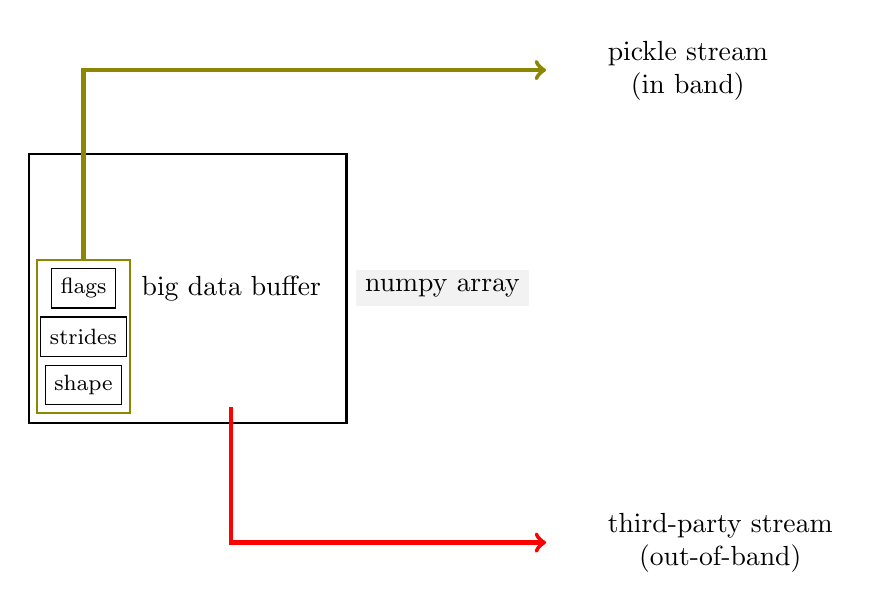
\begin{tikzpicture}
  \node[draw, rectangle,             align=center, minimum height=0.5cm] (1)
      {\footnotesize shape};
  \node[draw, rectangle, above=0.1cm of 1, align=center, minimum height=0.5cm] (2)
      {\footnotesize strides};
  \node[draw, rectangle, above=0.1cm of 2, align=center, minimum height=0.5cm] (3)
      {\footnotesize flags};
  \node[alt=<3>{draw=red, thick}{draw=black}, rectangle, right=0.2cm of 3, align=center, minimum height=3cm] (4)
      {big data buffer};
  \node[draw, thick, inner sep=0.2cm,fit=(4) (4) (1) (4)] (nparray) {};
  \node[align=left, fill=gray!10, right=0.1cm of nparray] (legend)  {numpy array};
  \node[visible on =<2->,draw=olive, thick, inner sep=0.1cm, fit=(1) (1) (1) (3), rectangle]  (metadata){};
  \node (picklestream) at (6, 4) {};
  \node (thirdpartystream) at (6, -2) {};
  \draw[visible on =<2->,color=olive, ->, ultra thick] (metadata.north) |- (picklestream);
  \draw[visible on=<3->,color=red, ->, ultra thick] (4.south) |- (thirdpartystream);
  \node[visible on =<2->,right=0.2cm of picklestream] (legend-picklestream) {%
     \begin{tabular}{c}
      pickle stream \\(in band)
      \end{tabular}};
  \node[visible on =<3->,right=0.2cm of thirdpartystream] (legend-thirdpartystream) {%
     \begin{tabular}{c}
      third-party stream \\(out-of-band)
      \end{tabular}};
    \node (void) at (6, 3) {};
        \end{tikzpicture}
\end{frame}

\begin{frame}[fragile]{Conclusion}
        \begin{tabular}{m{0.5cm} m{10cm}}
            \includegraphics[width=\linewidth] {media/rocket-emoji.png} &
        parallel computing often generates significant speedups when
            executing machine learning code \\
                                                                        & \\
        \end{tabular}
        \uncover<2->{
        \begin{tabular}{m{0.5cm} m{10cm}}
            \includegraphics[width=\linewidth] {media/thinking-face-emoji.png} &
        which backend (processes vs. threads) to use can be a
            problem-specific question: what's the size of your data, does your
            compute-hungry code releases the GIL... \\
                                                                        & \\
        \end{tabular}
        }
        \uncover<3->{
        \begin{tabular}{m{0.5cm} m{10cm}}
            \includegraphics[width=\linewidth] {media/arrow_up-emoji.png} &
            \textbf{working with upstream is worth the hassle}
        \end{tabular}
        \begin{flushright}
            Questions?
        \end{flushright}
        }
\end{frame}
\end{document}
